\section{Resultados}\label{sec:Results}

Os resultados referem-se às seis temporadas de teste da validação progressiva, de 2019 a 2024, com 380 partidas cada. Na previsão da média, a referência é a média da liga, isto é, a previsão ingênua descrita na Seção~\ref{subsec:Modelos}; na previsão probabilística, é a frequência de partidas acima da linha no treino. Os intervalos de confiança de 95\% vêm do \textit{bootstrap} por blocos de rodada. A Seção~\ref{subsec:ResReferencias} acrescenta, como análise de robustez posterior, a comparação com duas referências mais fortes que a média da liga.

\subsection{Dispersão das contagens}\label{subsec:ResDispersao}

Na regressão de Poisson sem penalização, a estatística de Pearson dividida pelos graus de liberdade ficou entre 0,96 e 0,98 nos gols e entre 1,18 e 1,25 nos escanteios, nas seis dobras. Os gols, portanto, não mostram sobredispersão em relação à distribuição de Poisson, enquanto os escanteios passam do limite de 1,1 fixado na Seção~\ref{subsec:Modelos}, o que levou ao ajuste da binomial negativa para esse alvo. O parâmetro $\alpha$ da binomial negativa, estimado nas previsões de validação de cada dobra, confirma a diferença: nos escanteios, ficou entre 0,017 e 0,027 em todos os modelos; nos gols, ficou abaixo de 0,02 e, em boa parte das dobras, chegou ao limite inferior da estimação, praticamente zero, o que torna a binomial negativa equivalente à Poisson.

\subsection{Comparação dos modelos}\label{subsec:ResComparacao}

A Tabela~\ref{tab:comparacao} resume o desempenho de cada modelo nas 2.280 partidas de teste. Nos gols, o Random Forest obteve a menor desviância média, 1,0574, contra 1,0759 da média da liga, uma redução de 0,0185, cerca de 1,7\%, com intervalo de confiança que não contém o zero. O XGBoost também superou a média da liga com significância, com redução de 0,0161. O Poisson \textit{ridge} reduziu a desviância em 0,0048, sem significância, e foi superado pelo Random Forest: a diferença entre os dois, de 0,0137 a favor do Random Forest, tem intervalo de 0,0027 a 0,0258. A diferença entre o Random Forest e o XGBoost, de 0,0025, não foi significativa (intervalo de $-0{,}0027$ a 0,0078), e a média simples das duas árvores praticamente coincidiu com o Random Forest.

\begin{table}[htb]
\IBGEtab{%
  \caption{Desempenho dos modelos nas temporadas de teste (2019--2024)}\label{tab:comparacao}
}{%
  \small
  \begin{tabular}{lccccc}
    \toprule
    Modelo & Desviância & $\Delta$ & IC95\% de $\Delta$ & MAE & RMSE \\
    \midrule
    \multicolumn{6}{l}{\textit{Gols}} \\
    Média da liga & 1,0759 & -- & -- & 1,208 & 1,524 \\
    Poisson \textit{ridge} & 1,0712 & $-$0,0048 & [$-$0,0201; 0,0111] & 1,201 & 1,519 \\
    Random Forest & 1,0574 & $-$0,0185 & [$-$0,0315; $-$0,0061] & 1,191 & 1,509 \\
    XGBoost & 1,0599 & $-$0,0161 & [$-$0,0278; $-$0,0054] & 1,193 & 1,511 \\
    Média RF e XGBoost & 1,0574 & $-$0,0185 & [$-$0,0308; $-$0,0075] & 1,192 & 1,509 \\
    Combinação ponderada & 1,0659 & $-$0,0100 & [$-$0,0241; 0,0039] & 1,196 & 1,515 \\
    \midrule
    \multicolumn{6}{l}{\textit{Escanteios}} \\
    Média da liga & 1,1838 & -- & -- & 2,790 & 3,499 \\
    Poisson \textit{ridge} & 1,1750 & $-$0,0088 & [$-$0,0161; $-$0,0017] & 2,782 & 3,486 \\
    Random Forest & 1,1744 & $-$0,0094 & [$-$0,0195; 0,0001] & 2,775 & 3,485 \\
    XGBoost & 1,1751 & $-$0,0087 & [$-$0,0157; $-$0,0024] & 2,782 & 3,486 \\
    Média RF e XGBoost & 1,1731 & $-$0,0106 & [$-$0,0184; $-$0,0034] & 2,777 & 3,483 \\
    Combinação ponderada & 1,1751 & $-$0,0087 & [$-$0,0186; 0,0008] & 2,776 & 3,486 \\
    \bottomrule
  \end{tabular}%
}{%
  \fonte{Elaborada pelo autor (2026).}
  \nota{Desviância de Poisson média por partida. $\Delta$: diferença de desviância em relação à média da liga (negativa quando o modelo erra menos). IC95\%: intervalo de confiança por \textit{bootstrap} com reamostragem de rodadas inteiras.}
}
\end{table}

Nos escanteios, as margens foram menores. A maior redução veio da média simples entre o Random Forest e o XGBoost, de 0,0106, cerca de 0,9\% da desviância da média da liga, com significância. O Poisson \textit{ridge} e o XGBoost também superaram a média da liga com significância, com reduções de 0,0088 e 0,0087. O Random Forest isolado reduziu a desviância em 0,0094, mas o limite superior do intervalo ficou ligeiramente acima de zero, 0,0001, de modo que a melhora não é significativa ao nível de 5\%. Entre os modelos, nenhuma diferença foi significativa: o Poisson \textit{ridge} ficou a 0,0006 do Random Forest (intervalo de $-0{,}0061$ a 0,0073), e a média das árvores, a $-0{,}0012$ (intervalo de $-0{,}0047$ a 0,0024). O MAE e o RMSE levam à mesma leitura: todos os modelos ficam abaixo da média da liga, e as diferenças entre eles aparecem só na terceira casa decimal.

Por temporada, o Random Forest teve desviância menor que a da média da liga nas seis temporadas de teste, nos dois alvos. A variação entre temporadas, porém, é maior que a diferença entre os modelos, como mostra a Figura~\ref{fig:temporadas}: a desviância da média da liga nos gols foi de 0,937 em 2024 a 1,164 em 2021, e nos escanteios, de 1,070 em 2024 a 1,397 em 2019. Nos escanteios, a desviância caiu de 2019 a 2022 em todos os modelos, e as curvas dos modelos quase se sobrepõem à da média da liga.

\begin{figure}[htb]
  \caption{Desviância média por partida em cada temporada de teste}\label{fig:temporadas}
  \centering
  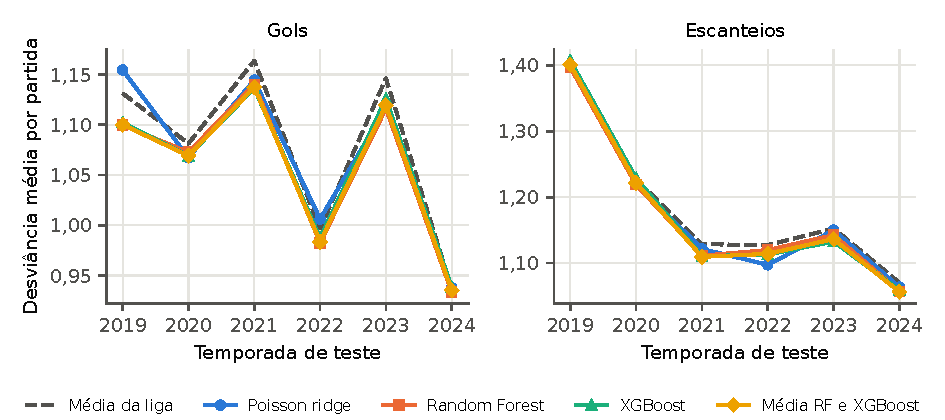
\includegraphics[width=\textwidth]{figures/deviance_temporadas.pdf}
  \fonte{Elaborada pelo autor (2026).}
\end{figure}

A combinação ponderada das previsões não superou o melhor modelo isolado em nenhum dos alvos. Nos gols, a validação interna atribuiu ao Poisson \textit{ridge} pesos de 0,3 a 1,0, e esse modelo foi o mais fraco dos três na temporada de teste; o resultado, 1,0659, ficou acima do Random Forest e sem diferença significativa em relação à média da liga. Nos escanteios, o Random Forest recebeu peso de 0,5 a 1,0 em cinco das seis dobras. A média simples das duas árvores, definida depois de vistos os resultados de teste das duas e antes do resultado dela, ficou igual ao Random Forest nos gols até a quarta casa decimal (diferença com intervalo de $-0{,}0026$ a 0,0027) e foi a melhor previsão nos escanteios, sem diferença significativa em relação ao Random Forest.

As escolhas feitas na validação interna variaram entre as dobras. O peso da referência na Equação~(\ref{eq:enc}) foi $k = 1.000$, o maior valor da grade, em três das doze dobras (gols em 2020 e 2021, escanteios em 2019). Com um peso tão alto, a média da temporada se reduz à referência, isto é, à média final da equipe na temporada anterior, o que é um limite natural da grade. Nos escanteios, o $k$ escolhido caiu a cada temporada, de 1.000 em 2019 para 10 em 2024. Nos gols, os \textit{pi-ratings} e os índices GAP entraram com a fração 1 em todas as dobras; nos escanteios, a fração dos \textit{pi-ratings} foi 0,5 em cinco das seis. As árvores escolhidas foram rasas: o Random Forest usou profundidade 1 nas quatro primeiras dobras dos gols e profundidade de 1 a 4 em todas as dobras dos escanteios.

\subsection{Referências mais fortes que a média da liga}\label{subsec:ResReferencias}

A média da liga é uma constante por temporada de teste e não acompanha o nível de cada temporada, que nos escanteios varia de 10,16 por partida em 2024 a 11,03 em 2022. Esta análise de robustez foi feita depois dos resultados anteriores e não estava planejada; o peso de 100 partidas da média corrente (Seção~\ref{subsec:Modelos}) foi fixado sem ajuste. A Tabela~\ref{tab:referencias} compara os modelos com a média da temporada anterior e com a média corrente da liga.

\begin{table}[htb]
\IBGEtab{%
  \caption{Comparação com referências mais fortes que a média da liga (2019--2024)}\label{tab:referencias}
}{%
  \scriptsize\setlength{\tabcolsep}{2pt}%
  \begin{tabular}{lccccc}
    \toprule
    & Desv. & $\Delta$ (ant.) & IC95\% & $\Delta$ (corr.) & IC95\% \\
    \midrule
    \multicolumn{6}{l}{\textit{Gols}} \\
    Ref.: temporada anterior & 1,0813 & -- & -- & -- & -- \\
    Ref.: corrente da liga & 1,0761 & -- & -- & -- & -- \\
    Média da liga & 1,0759 & $-$0,0053 & [$-$0,0106; 0,0004] & $-$0,0001 & [$-$0,0045; 0,0044] \\
    Poisson \textit{ridge} & 1,0712 & $-$0,0101 & [$-$0,0253; 0,0059] & $-$0,0049 & [$-$0,0196; 0,0108] \\
    Random Forest & 1,0574 & $-$0,0239 & [$-$0,0375; $-$0,0102] & $-$0,0187 & [$-$0,0314; $-$0,0067] \\
    XGBoost & 1,0599 & $-$0,0214 & [$-$0,0348; $-$0,0090] & $-$0,0162 & [$-$0,0282; $-$0,0052] \\
    Média RF e XGBoost & 1,0574 & $-$0,0239 & [$-$0,0370; $-$0,0109] & $-$0,0186 & [$-$0,0309; $-$0,0072] \\
    \midrule
    \multicolumn{6}{l}{\textit{Escanteios}} \\
    Ref.: temporada anterior & 1,1895 & -- & -- & -- & -- \\
    Ref.: corrente da liga & 1,1792 & -- & -- & -- & -- \\
    Média da liga & 1,1838 & $-$0,0057 & [$-$0,0121; 0,0010] & 0,0045 & [$-$0,0035; 0,0122] \\
    Poisson \textit{ridge} & 1,1750 & $-$0,0145 & [$-$0,0237; $-$0,0057] & $-$0,0043 & [$-$0,0124; 0,0040] \\
    Random Forest & 1,1744 & $-$0,0151 & [$-$0,0260; $-$0,0046] & $-$0,0049 & [$-$0,0160; 0,0058] \\
    XGBoost & 1,1751 & $-$0,0144 & [$-$0,0233; $-$0,0057] & $-$0,0041 & [$-$0,0134; 0,0047] \\
    Média RF e XGBoost & 1,1731 & $-$0,0164 & [$-$0,0258; $-$0,0075] & $-$0,0061 & [$-$0,0157; 0,0031] \\
    \bottomrule
  \end{tabular}%
}{%
  \fonte{Elaborada pelo autor (2026).}
  \nota{Desviância (Desv.) de Poisson média por partida. $\Delta$ (ant.) e $\Delta$ (corr.): diferença de desviância do modelo em relação à média da temporada anterior e à média corrente da liga, respectivamente (negativa quando o modelo erra menos). IC95\%: \textit{bootstrap} por blocos de rodada. A média corrente usa o peso de 100 partidas, fixado sem ajuste e depois de vistos os demais resultados.}
}
\end{table}

Nos gols, o resultado se mantém. O Random Forest reduz a desviância em 0,0239 contra a média da temporada anterior e em 0,0187 contra a média corrente, e o XGBoost e a média das duas árvores também, todos com intervalos que não contêm o zero; a média corrente (1,0761) não é melhor que a média da liga (1,0759). Nos escanteios, a conclusão muda. Contra a média da temporada anterior, todos os modelos seguem melhores com significância. Contra a média corrente, que por si só já reduz a desviância da média da liga em 0,0046 (1,1792 contra 1,1838), nenhum modelo tem ganho significativo: o melhor, a média do Random Forest e do XGBoost, fica 0,0061 abaixo, com intervalo de $-0{,}0157$ a 0,0031. Quase metade do ganho aparente sobre a média da liga (0,0046 de 0,0106) vem, portanto, de acompanhar o nível da temporada, e não de distinguir uma partida da outra.

\subsection{Bootstrap por blocos e comparação com as rodadas anteriores}\label{subsec:ResBlocos}

Nas rodadas anteriores da modelagem, os intervalos foram calculados por \textit{bootstrap} de partidas isoladas. Refeitos com a reamostragem de rodadas inteiras, nenhum resultado mudou de conclusão. O Poisson \textit{ridge} da segunda rodada, com $k = 5$ fixo, continuou superior à média da liga nos escanteios, com intervalo de $-0{,}0148$ a $-0{,}0021$ por partida e de $-0{,}0151$ a $-0{,}0023$ por rodada, e continuou sem significância nos gols. O Random Forest da terceira rodada, com a grade menor de hiperparâmetros, seguiu significativo nos dois alvos: nos gols, o intervalo passou de $[-0{,}0286; -0{,}0068]$ para $[-0{,}0293; -0{,}0066]$, e nos escanteios, de $[-0{,}0240; -0{,}0032]$ para $[-0{,}0254; -0{,}0042]$. O XGBoost da terceira rodada não se distinguiu da média da liga em nenhum dos dois esquemas. Os intervalos por rodada ficaram pouco mais largos que os por partida, o que indica dependência fraca entre as partidas de uma mesma rodada. A ampliação das grades na rodada final não melhorou o Random Forest: a diferença entre a versão final e a da terceira rodada foi de $-0{,}0007$ nos gols e de 0,0048 nos escanteios, ambas sem significância. O ganho da rodada final veio do XGBoost, que passou de 1,0685 para 1,0599 nos gols e de 1,1866 para 1,1751 nos escanteios e, com isso, a superar a média da liga nos dois alvos.

A significância dos escanteios, porém, não foi estável entre as execuções (Tabela~\ref{tab:instabilidade}). O Random Forest foi significativo na terceira rodada, ficou no limite na 4b (limite superior de $-0{,}00003$) e deixou de ser na 4c. O XGBoost não foi significativo na terceira rodada, foi na 4b e na 4c e deixou de ser na 4d, em que a busca foi ampliada. A média do Random Forest e do XGBoost foi significativa na 4b e na 4c e não na 4d. Há cinco previsões por alvo, quatro execuções e nenhuma correção para comparações múltiplas; a escolha da 4c como final foi feita depois de ver o teste da 4d (Seção~\ref{subsec:DiscLimitacoes}).

\begin{table}[htb]
\IBGEtab{%
  \caption{Intervalos de confiança de $\Delta$ nos escanteios, em relação à média da liga, por execução}\label{tab:instabilidade}
}{%
  \small
  \begin{tabular}{lccc}
    \toprule
    Execução & Random Forest & XGBoost & Média RF e XGBoost \\
    \midrule
    Rodada 3 & [$-$0,0254; $-$0,0042]\textsuperscript{*} & [$-$0,0142; 0,0198] & -- \\
    Rodada 4b & [$-$0,0197; $-$0,00003]\textsuperscript{*} & [$-$0,0155; $-$0,0005]\textsuperscript{*} & [$-$0,0183; $-$0,0030]\textsuperscript{*} \\
    Rodada 4c (final) & [$-$0,0195; 0,0001] & [$-$0,0157; $-$0,0024]\textsuperscript{*} & [$-$0,0184; $-$0,0034]\textsuperscript{*} \\
    Rodada 4d & [$-$0,0195; 0,0001] & [$-$0,0103; 0,0073] & [$-$0,0156; 0,0016] \\
    \bottomrule
  \end{tabular}%
}{%
  \fonte{Elaborada pelo autor (2026).}
  \nota{IC95\% por \textit{bootstrap} de blocos de rodada. *: intervalo que não contém o zero. A média de RF e XGBoost só foi calculada a partir da rodada 4b. O Random Forest da 4d é o da 4c: só a busca do XGBoost foi ampliada.}
}
\end{table}

\subsection{Previsão probabilística}\label{subsec:ResProbabilistica}

Nas temporadas de teste, 43,7\% das partidas tiveram mais de 2,5 gols, e 57,1\% tiveram mais de 9,5 escanteios. A Tabela~\ref{tab:probabilistica} compara as probabilidades obtidas pela Poisson e pela binomial negativa com a frequência dessas partidas nas temporadas de treino. Todos os valores de perda logarítmica ficaram entre 0,680 e 0,687, próximos de $\ln 2 \approx 0{,}693$, que é a perda de quem atribui probabilidade de 50\% a todas as partidas.

\begin{table}[htb]
\IBGEtab{%
  \caption{Previsão de mais de 2,5 gols e de mais de 9,5 escanteios (2019--2024)}\label{tab:probabilistica}
}{%
  \footnotesize\setlength{\tabcolsep}{4pt}%
  \begin{tabular}{llcccc}
    \toprule
    Média prevista por & Distribuição & Perda log. & IC95\% de $\Delta$ & Brier & IC95\% de $\Delta$ \\
    \midrule
    \multicolumn{6}{l}{\textit{Mais de 2,5 gols}} \\
    Frequência no treino & -- & 0,6870 & -- & 0,2469 & -- \\
    Média da liga & Poisson & 0,6865 & [$-$0,0010; 0,0001] & 0,2467 & [$-$0,0005; 0,0001] \\
    Média da liga & Binomial neg. & 0,6866 & [$-$0,0009; 0,0002] & 0,2467 & [$-$0,0004; 0,0001] \\
    Poisson \textit{ridge} & Poisson & 0,6857 & [$-$0,0080; 0,0058] & 0,2460 & [$-$0,0042; 0,0024] \\
    Poisson \textit{ridge} & Binomial neg. & 0,6857 & [$-$0,0080; 0,0058] & 0,2460 & [$-$0,0042; 0,0024] \\
    Random Forest & Poisson & 0,6804 & [$-$0,0120; $-$0,0015] & 0,2436 & [$-$0,0059; $-$0,0007] \\
    Random Forest & Binomial neg. & 0,6804 & [$-$0,0119; $-$0,0015] & 0,2436 & [$-$0,0059; $-$0,0008] \\
    XGBoost & Poisson & 0,6809 & [$-$0,0108; $-$0,0018] & 0,2439 & [$-$0,0053; $-$0,0009] \\
    XGBoost & Binomial neg. & 0,6809 & [$-$0,0107; $-$0,0018] & 0,2439 & [$-$0,0053; $-$0,0009] \\
    \midrule
    \multicolumn{6}{l}{\textit{Mais de 9,5 escanteios}} \\
    Frequência no treino & -- & 0,6842 & -- & 0,2455 & -- \\
    Média da liga & Poisson & 0,6869 & [0,0005; 0,0049] & 0,2468 & [0,0002; 0,0023] \\
    Média da liga & Binomial neg. & 0,6845 & [$-$0,0004; 0,0010] & 0,2457 & [$-$0,0002; 0,0005] \\
    Poisson \textit{ridge} & Poisson & 0,6869 & [$-$0,0007; 0,0060] & 0,2468 & [$-$0,0003; 0,0028] \\
    Poisson \textit{ridge} & Binomial neg. & 0,6841 & [$-$0,0024; 0,0022] & 0,2455 & [$-$0,0011; 0,0010] \\
    Random Forest & Poisson & 0,6863 & [$-$0,0019; 0,0060] & 0,2465 & [$-$0,0009; 0,0028] \\
    Random Forest & Binomial neg. & 0,6837 & [$-$0,0037; 0,0024] & 0,2453 & [$-$0,0018; 0,0012] \\
    XGBoost & Poisson & 0,6855 & [$-$0,0022; 0,0044] & 0,2461 & [$-$0,0011; 0,0021] \\
    XGBoost & Binomial neg. & 0,6830 & [$-$0,0036; 0,0010] & 0,2449 & [$-$0,0018; 0,0004] \\
    \bottomrule
  \end{tabular}%
}{%
  \fonte{Elaborada pelo autor (2026).}
  \nota{$\Delta$: diferença em relação à frequência de partidas acima da linha nas temporadas de treino (negativa quando a previsão é melhor). IC95\%: \textit{bootstrap} por blocos de rodada.}
}
\end{table}

Nos gols, o Random Forest e o XGBoost superaram a frequência com significância nas duas métricas: o Random Forest reduziu a perda logarítmica em 0,0066 e o escore de Brier em 0,0033. As probabilidades pela Poisson e pela binomial negativa praticamente coincidem, como esperado pelo $\alpha$ próximo de zero. Nos escanteios, nenhuma previsão superou a frequência. A binomial negativa foi melhor que a Poisson em todos os modelos, e a média da liga com a Poisson foi a única previsão significativamente pior que a frequência: com a variância subestimada, a Poisson concentra a probabilidade perto da média e distorce a chance de passar da linha.

A Figura~\ref{fig:calibracao} mostra a calibração das probabilidades do Random Forest com a binomial negativa, agrupando as partidas de teste em decis da probabilidade prevista. Nos gols, as probabilidades foram de 0,36 a 0,56 na média dos decis. Nos três decis mais altos, a frequência observada acompanhou a prevista; nos decis mais baixos, entre 0,36 e 0,41, ela oscilou entre 0,33 e 0,44 sem seguir a ordem das previsões. Nos escanteios, as probabilidades ficaram concentradas entre 0,52 e 0,65, e a frequência observada variou pouco entre os decis, quase sempre abaixo da prevista: a média das previsões, 59,2\%, ficou acima dos 57,1\% observados. O modelo, portanto, distingue pouco as partidas com mais e menos escanteios, o que é coerente com a ausência de ganho sobre a frequência.

\begin{figure}[htb]
  \caption{Calibração das probabilidades do Random Forest com a binomial negativa (2019--2024)}\label{fig:calibracao}
  \centering
  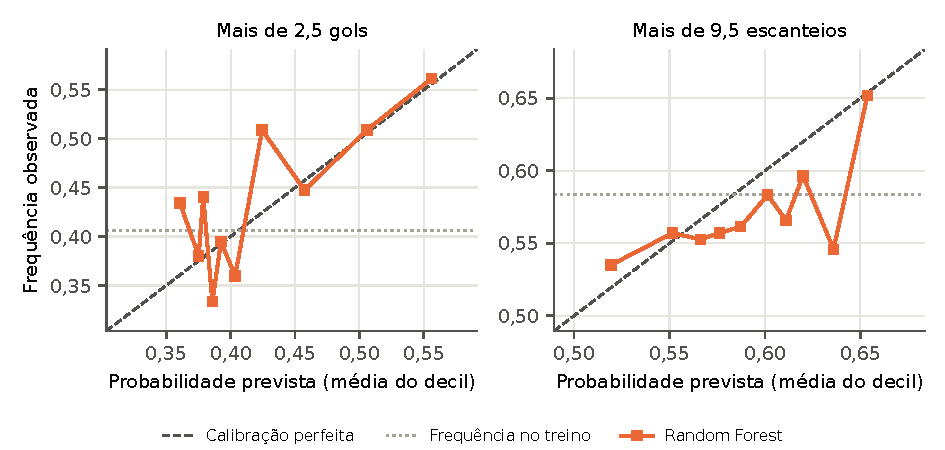
\includegraphics[width=\textwidth]{figures/calibracao.pdf}
  \fonte{Elaborada pelo autor (2026).}
  \nota{Cada ponto é um decil da probabilidade prevista, com cerca de 228 partidas: no eixo horizontal, a probabilidade média prevista; no vertical, a proporção de partidas acima da linha. A linha pontilhada é a frequência média no treino.}
\end{figure}

\subsection{Importância das variáveis}\label{subsec:ResImportancia}

A Tabela~\ref{tab:importancia} apresenta a importância por permutação de cada grupo de variáveis no Random Forest e no XGBoost, como a média das seis temporadas de teste. A do Poisson \textit{ridge} não é apresentada: nesse modelo, as variáveis dos \textit{pi-ratings} e dos índices GAP são muito correlacionadas e recebem coeficientes de sinais opostos, e a permutação do grupo desfaz essa compensação, o que infla a importância medida sem refletir a contribuição das variáveis.

\begin{table}[htb]
\IBGEtab{%
  \caption{Importância por permutação por grupo de variáveis (2019--2024)}\label{tab:importancia}
}{%
  \small
  \begin{tabular}{lcccc}
    \toprule
    & \multicolumn{2}{c}{Gols} & \multicolumn{2}{c}{Escanteios} \\
    \cmidrule(lr){2-3}\cmidrule(lr){4-5}
    Grupo & RF & XGBoost & RF & XGBoost \\
    \midrule
    Índices GAP & 0,0101 & 0,0086 & 0,0011 & 0,0018 \\
    \textit{Pi-ratings} & 0,0074 & 0,0076 & 0,0008 & 0,0016 \\
    Média da temporada & $-$0,0006 & 0,0012 & 0,0070 & 0,0028 \\
    Forma recente & 0,0001 & $-$0,0005 & 0,0042 & 0,0033 \\
    Técnico & 0,0006 & 0,0013 & 0,0001 & 0,0006 \\
    Dias de descanso & 0,0007 & $-$0,0012 & 0,0001 & $-$0,0003 \\
    Sem público & 0,0000 & 0,0000 & 0,0000 & 0,0001 \\
    Equipe promovida\textsuperscript{a} & -- & $-$0,0002 & -- & 0,0001 \\
    Formação\textsuperscript{b} & -- & -- & 0,0000 & 0,0001 \\
    \bottomrule
  \end{tabular}%
}{%
  \fonte{Elaborada pelo autor (2026).}
  \nota{Aumento médio da desviância de Poisson ao embaralhar o grupo na temporada de teste, em 20 repetições, média das seis dobras; valores negativos indicam que o embaralhamento não piorou a previsão. Valores com módulo menor que 0,00005 aparecem como 0,0000. (a) Só no XGBoost. (b) Só nos escanteios e só nas dobras de 2019 a 2021, em que a formação foi escolhida na validação interna.}
}
\end{table}

Os dois alvos dependem de grupos diferentes. Nos gols, a contribuição vem dos índices de força: os índices GAP e os \textit{pi-ratings} somam quase toda a importância nas duas árvores, enquanto a média da temporada e a forma recente ficam próximas de zero ou negativas, provavelmente porque a informação delas já está contida nos índices. Nos escanteios, o grupo mais importante no Random Forest é a média da temporada, seguida pela forma recente; no XGBoost, a forma recente vem à frente, seguida pela média da temporada, e os índices GAP de escanteios aparecem logo depois. Os \textit{pi-ratings}, que medem a diferença de força em saldo de gols, contribuem pouco para os escanteios. Técnico, dias de descanso, partidas sem público e equipe promovida têm importância próxima de zero nos dois alvos. Os valores SHAP do XGBoost apontam na mesma direção: nos gols, a maior contribuição média absoluta é a dos índices GAP, e nos escanteios, a da forma recente.

A formação tática da partida-alvo não melhorou a previsão dos escanteios. Na validação interna, ela foi escolhida em três das seis dobras, de 2019 a 2021, sempre pelo número de jogadores do meio-campo para a frente, e nunca pelas famílias de amplitude; de 2022 em diante, o conjunto escolhido não a incluiu. Nas três dobras em que entrou, a importância por permutação foi nula no Random Forest, que não chegou a usar a variável nas divisões, e de 0,0001 em média no XGBoost, com o maior valor, 0,0003, em 2021. A contribuição média absoluta pelos valores SHAP também ficou na ordem de $10^{-4}$.
